\documentclass[12pt]{article}
% \textwidth 15.5cm \oddsidemargin 0cm \topmargin -2cm \textheight
% 24cm \footskip 1cm
\usepackage[british]{babel}
\usepackage{epsfig}
\usepackage{amsmath,graphicx,psfrag,pstricks,float,amssymb,fancyhdr,pdfpages, hyperref, enumitem, listings, subfig, diagbox, appendix, lastpage, bm}
\usepackage[backend=biber]{biblatex}
% \usepackage[sorting=none]{biblatex}
\usepackage[margin=25mm]{geometry}
%\usepackage{minted}

\DeclareMathOperator*{\argmax}{argmax}
\DeclareMathOperator*{\argmin}{argmin}

% \pagestyle{fancy}
% \pagenumbering{arabic}
% \fancyhead[L]{}
% \cfoot{\thepage}
\fancypagestyle{technical_abstract}{
  \fancyhf{}
  \fancyfoot[C]{Page \thepage}
}

\fancypagestyle{default}{
  \fancyhf{}
  \fancyfoot[C]{Page \thepage\ of \pageref{LastPage}}
}

\pagestyle{fancy}

% \setlength{\headheight}{15pt}
\renewcommand{\headrulewidth}{0pt}
\linespread{1.3}  % "One-and-a-half" spacing

\def\n{\noindent}
\def\u{\underline}
\def\hs{\hspace}
\newcommand{\thrfor}{.^{\displaystyle .} .}
%\newcommand{\bvec}[1]{{\bf #1}}

\addbibresource{bibliography.bib}

\begin{document}

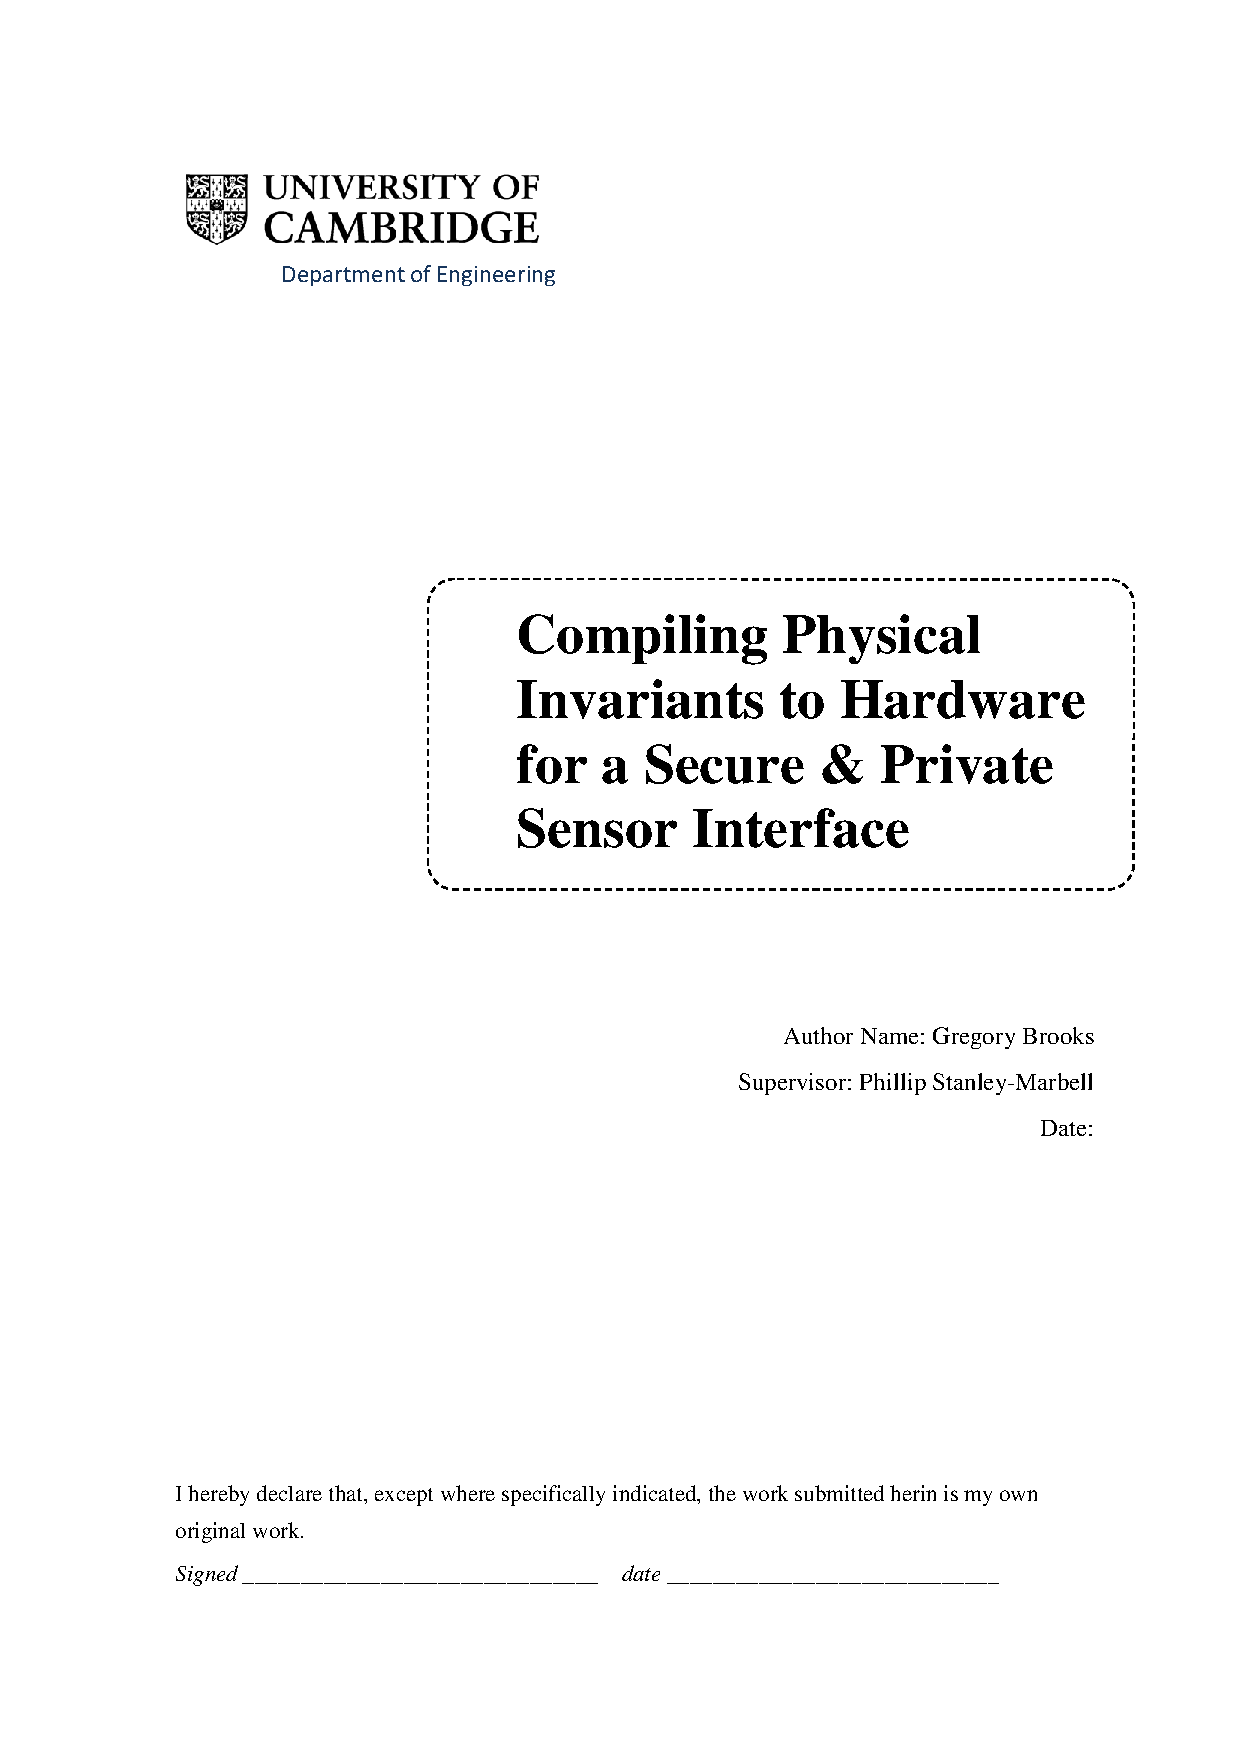
\includepdf[pages={1}]{coversheet.pdf}
\clearpage \mbox{}
\pagenumbering{gobble}
\clearpage
\pagenumbering{arabic}

\noindent

%
% TITLE & CONTENTS PAGE
%

\title
{
  IIB Project Report:\\
  Compiling Physical Invariants to Hardware for a Secure \& Private Sensor Interface\\
}
\author{Gregory Brooks, gb510, Christ's College}
\date{29 May 2019}
\maketitle

\tableofcontents

\pagenumbering{gobble}
\clearpage
\pagenumbering{arabic}

%
% TECHNICAL ABSTRACT
%
\pagestyle{technical_abstract}
\section{Technical Abstract}

\begin{center}
{
  \bf Compiling Physical Invariants to Hardware for a Secure \& Private Sensor Interface\\
}
Gregory Brooks, gb510, Christ's College
\end{center}
\rule{15.7cm}{0.5mm}
\vspace{1cm}

\textit{$\langle$ TODO: write this last$\rangle$}

This project investigates the idea of using the Newton~\cite{Newton} physics description language as part of a multi-sensor embedded local differential privacy system implemented on an iCE40 FPGA.
\textit{$\langle$ TODO: tidy up the above and expand on it if necessary$\rangle$}

  %
  % SYSTEM DIAGRAM
  %

  \subsection{System Diagram}
    \textit{$\langle$ TODO: insert block diagram of system and describe which parts have been the focus of this project$\rangle$}


\newpage


\pagestyle{default}
%
% INTRODUCTION
%

\section{Introduction}

  \textit{Differential privacy} can be thought of as a constraint applied to queries for information from a database whereby information about individual members of the database is obscured whilst still releasing useful aggregate information about a population/demographic as a whole. A simple method of implementing this would be the addition of zero mean noise to database entries --- whilst the noise would obscure the \textit{true} value of individual data points, the mean value of the dataset would remain intact. More formally, \textit{$\epsilon$-differential privacy} is defined by Dwork and Smith~\cite{dwork2010differential} as follows:\\
  \\
  ``A randomized function K gives \textit{$\epsilon$-differential privacy} if for all data sets $x$ and $x'$ differing on at most one element, and all $S \subseteq Range(K)$,
  \begin{equation}
    Pr[K(x) \in S] \leq exp(\epsilon) \times Pr[K(x') \in S],
  \end{equation}
  where the probability space in each case is over the coin flips of the mechanism K.''\\

  Throughout this project, the chosen randomised function K is the Laplace mechanism i.e. the addition of zero mean Laplace distributed random noise to \textit{private} data such as a measurement from a sensor\footnote{the \textit{databases} in this scenario are simply single sensor measurements hence any two \textit{databases} will always differ by at most a single element.} to produce a \textit{noised output} that can be released to untrusted observers (the outside world). This technique provides privacy by ensuring that every possible measurement value (i.e. any value within the sensor measurement range) has a similar posterior probability of being the \textit{true private} value given the observed \textit{noised output}. An outside observer can use the \textit{noised output} to estimate the value of \textit{private} data with some uncertainty but should never be able to deduce it with complete certainty.\\

  The Laplace distribution used by this method has parameter $\frac{\lambda}{\epsilon}$. $\lambda$ refers to the \textit{global sensitivity} of the database query function; in this scenario this is simply the maximum difference between possible sensor measurements i.e. a sensor's measurement range. $\epsilon$ is a privacy scaling parameter, where a smaller $\epsilon$ value results in greater privacy by applying noise with a greater variance, thereby reducing the amount of information each \textit{noised output} value reveals about the \textit{private} data. For a particular application, deciding on an $\epsilon$ value is a tradeoff between utility and privacy since, in the limiting case, an $\epsilon$ value of zero means that the system outputs no useful information (just random noise), consequently keeping the \textit{private} data completely private.\\

  Within the context of embedded electronic systems, recent work (for example, this project builds heavily on the work of Choi et al.~\cite{Choi2018GuaranteeingLD}) has investigated the implementation of differential privacy techniques on low power hardware such as the processors found in smartphones and Internet-of-Things devices. In contrast to the conventional differential privacy model, where a trusted database stores \textit{private} data collected from local hardware, a local differential privacy architecture involves \textit{private} data being masked at the source (e.g. an embedded sensor system) before being sent to an untrusted database~\cite{Kairouz:2014}. This local approach can result in a more secure system since \textit{private} data does not need to be recorded anywhere nor transmitted from local hardware to a remote server.\\

  One challenge associated with implementing local differential privacy is that the randomised function K used to mask \textit{private} data can be difficult to implement on low power hardware --- one of the findings presented by Choi et al.~\cite{Choi2018GuaranteeingLD} is that a finite precision implementation of the Laplace mechanism can lead to infinite privacy loss, since certain specific values for \textit{noised output} data can reveal the \textit{true} values for \textit{private} unnoised data with complete certainty. This problem is most apparent on low power hardware utilising low precision fixed point arithmetic. \textit{$\langle$ TODO: finish this paragraph (and introduction section e.g. talk about Newton and multi sensor)$\rangle$}\\


\newpage



%
% THEORETICAL DEVELOPMENT
%

\section{Theoretical Development}
  The early stages of the project involved investigating potential research problems that would involve compiling Newton descriptions into a hardware description language. It soon became apparent that the Newton language was well suited to describing the relationships between sensors in a multi-sensor embedded system, thereby providing a basis to build upon the single-sensor state-of-the-art~\cite{Choi2018GuaranteeingLD}~\cite{diffpriv_2006}.
  \subsection{Brainstorming Example Applications}
    \subsubsection{Digital Camera/Viola-Jones Facial Detection}
      \textit{$\langle$ TODO $\rangle$}

    \subsubsection{Microphone}
      \textit{$\langle$ TODO $\rangle$}

    \subsubsection{\textit{Intelligent} Noising}
      \textit{$\langle$ TODO: allowing the compiler to choose how to add noise, rather than explicity stating where to add noise$\rangle$}
      This project investigates a system which allows a user to specify which measurement signals they wish to add random noise to. It is possible to generalise this idea to a hypothetical system which has control over how it applies random noise to measurement data in order to mask a more abstract form of information. One concrete example of this would be when working with images (e.g. the  Viola-Jones example above) --- given the requirement that individuals' identities should be obscured whilst still providing enough information for facial detection algorithms to work reliably, a system might choose to apply noise using, for example:

      \begin{itemize}
        \item Random noise added to pixel intensities.
        \item Convolution with a random filter.
        \item Random rearrangement of pixels.
        \item A combination of multiple techniques.
      \end{itemize}




  \subsection{System Specification}
    \textit{$\langle$ TODO: move to technical abstract?$\rangle$}

  \subsection{Multi-Sensor Differential Privacy Loss}

  \subsection{Privacy Budget Management System Architecture}
    In the following section, I propose a privacy management system architecture that could be used to manage multi-sensor privacy on an FPGA. Due to project time constraints, the system has not been completely implemented, since this would divert time and attention away from investigating the more important research questions posed by the project.
    \\
    \textit{$\langle$ TODO: describe what will have been implemented by the submission date e.g. use privacy yaml file and Newton AST to generate some of the logic implementation by filling in a Verilog template$\rangle$}
    \\
    The proposed system architecture is as follows:
    \begin{itemize}
      \item The FPGA acts as a sensor interface, allowing external circuitry to request noised sensor values. Noised measurement signals are referred to as \textit{protected}, as their true value has been masked by the addition of zero-mean Laplace distributed random noise to preseve privacy; the system also allows \textit{unprotected} signals to be forwarded to the outside world with no random noise added. %Newton also allows signals to be derived from other more fundamental signals e.g. a value derived from sensor measurements; for this system, random noise can only be applied to sensor measurement signals i.e. these are the only types of signal that can be (and the only types of signal that need to be) protected.
      \item A \textit{privacy file} (e.g. a YAML file) is used to specify protected measurement signals for a particular embedded system.
      \item In order to apply random noise to a particular signal, a range of parameters must be defined for each protected signal:
      \begin{itemize}
        \item Range of possible sensor outputs.
        \item \textit{Privacy budget} value allocated to the sensor.
        \item \textit{Privacy budget} replenishment rate.
        \item Value of $\epsilon$, a measure of privacy where a smaller value results in greater privacy by increasing the variance of applied noise~\cite{Choi2018GuaranteeingLD}.
      \end{itemize}
      These values can be provided for each protected signal within the \textit{privacy file}.
      \item The FPGA maintains a differential privacy \textit{budget} for each protected signal. Querying a value for a protected signal (i.e. requesting a noised measurement from the FPGA) causes that signal to incur a privacy loss. The FPGA quantifies this loss (a function of the random noise sample added to the raw measurement~\cite{Choi2018GuaranteeingLD}) and subtracts it from the signal's privacy budget. Once the budget is depleted, further queries of the signal in question are ignored --- a nonzero budget replenishment rate can be specified in the privacy file so that the signal can eventually be queried again once the budget has replenished sufficiently.
      \item Invariants in the Newton description define relationships between signals. This is important as privacy is lost if a measurand's value is calculated by taking measurements from related sensors, without directly measuring the measurand. The system must account for this \textit{indirect} privacy loss:
      \begin{itemize}
        \item Each Newton invariant containing protected measurement signals has an associated bitfield register on the FPGA. Each bit in the register acts as a read flag for each measurement signal contained in the associated invariant --- the flag is set when the sensor is queried (i.e. when a measurement is taken and the noised measurement value becomes \textit{known} to the outside world) and is not cleared until the sensor's privacy budget is completely replenished some time after a query (at which point the measurement value can be considered \textit{unknown} to the outside world).
        \item As long as any two flags remain unset, there are two variables in the equation that are \textit{unknown} to an attacker. The equation cannot be solved and so no information\footnote{This assumes that the probability distributions of sensor outputs are independent, see Appendix \ref{appendix:diff_priv_loss} for an investigation into correlated measurements.} can be gained about the \textit{unknown} values.
        \item If only one bit remains unset, then the remaining \textit{unknown} value can be calculated using the other \textit{known} values with set flags --- the \textit{unknown} signal incurs a privacy loss. If all flag bits are set then responding to a measurement query results in a privacy loss for every other signal in the invariant. These scenarios can be summarised by saying that, for signals contained within a particular Newton invariant, a signal experiences an indirect privacy loss if any of the other signals in the invariant are queried \textit{and} all other signals are \textit{known} i.e. have been recently queried.
        \item If responding to a query would exceed the privacy budget for any protected signal (not just the one being queried) then a response should not be granted.
      \end{itemize}
      \item The mathematics behind the calculation of a quantitative value for privacy loss is investigated in Appendix \ref{appendix:diff_priv_loss}; whilst calculation of an exact value for privacy loss (Equation \ref{eqn:exact_indirect_priv_loss} in Appendix \ref{appendix:diff_priv_loss}) requires the use of a mathematical optimisation technique such as Lagrange multipliers, a simpler calculation can be used to obtain an upper bound on the value. This simpler calculation can be performed more easily on a small FPGA such as the iCE40, and can even be pre-calculated during compile-time since it is a function of the random noise output only.

    \end{itemize}

\newpage



%
% TECHNOLOGIES AND TECHNIQUES USED
%

\section{Technologies and Techniques Used}
  \subsection{GitHub} \label{subsection:GitHub}
    Below is a list of GitHub repositories containing work done as part of this project:
    \begin{itemize}
        \item Main project repository containing Python simulations/tests, Verilog templates and C code to fill in templates:\\
        \url{https://github.com/Gregox273/Newton-Verilog-Compiler}
        \item Verilog repository for iCE40 differential I/O based uniform random number generator:\\
        \url{https://github.com/physical-computation/iCE40-LVDS-RNG}
        \item Schematic and PCB design for hardware (zener diode based) noise generator:\\
        \url{https://github.com/Gregox273/zener-rng}

    \end{itemize}
    \textit{$\langle$ TODO: describe how GitHub was used$\rangle$}
    \textit{$\langle$ TODO: include an example of commit history for a repository$\rangle$}

  \subsection{iCE40 FPGA}

  \subsection{Software Prototyping}

  \subsection{FPGA Synthesis Toolchain}

  \subsection{Repository Structure and Build System}

  \subsection{Verilog Development Techniques}
    \textit{$\langle$ TODO: describe good practices picked up over the course of this project$\rangle$}

\newpage



%
% DELIVERABLES
%

\section{Deliverables}
  \subsection{Hardware Entropy Source}
    One of the key components of a security/privacy application is a true random number generator (TRNG). Unlike a pseudorandom number generator (PRNG), which produces a predictable deterministic outcome, a true random number generator's output cannot be anticipated by an attacker, preserving system security and users' privacy. The output bit rate of TRNGs is often limited so can be used to seed a cryptographically secure PRNG (CSPRNG) algorithm to increase output bit rate without significantly compromising security. This extra step was not required for this project, since the rate at which random numbers are consumed is relatively low.\\

    Initial investigations focused on using the iCE40 FPGA's differential I/O hardware to generate random bits which could be fed into a TRNG to generate random samples from an arbitrary distribution. Initially, it was hoped that simply leaving two comparator inputs floating would cause the output to fluctuate randomly --- in practice this did not occur as the comparator hardware requires one of the inputs to be biased within a narrow common mode voltage range (roughly half the I/O supply voltage, allowing the other input to swing about this reference voltage)~\cite{ice40_diff_io}. I decided to design a PCB to set this bias voltage, as well as provide an alternative entropy source in the form of a reverse biased zener diode producing avalanche noise. In theory, this circuit would provide a better i.e. less predictable source of entropy since, unlike the floating input pin, the avalanche noise (and therefore random number output) produced is independent of the device's external environment\footnote{A floating input pin can easily be influenced by its external environment e.g. picking up 50Hz noise from nearby electrical mains, resulting in a non-uniform frequency spectrum for random output.}.\\

    The circuit used in this noise generator is based on a design by Professor Paul Horowitz~\cite[p.~984]{art_of_electronics}, modified to operate at 3.3V and 0V power rails (rather than $\pm5V$). Avalanche noise produced by a reverse biased zener diode is amplified through a dual op-amp amplifier stage before being modulated about a 1.65V DC bias $\left(\frac{V_{cc}}{2}\right)$; this output can then be fed into one of the iCE40's comparator inputs. A second output on the PCB comes from a simple potentiometer circuit to set the common mode reference voltage on the second comparator input (with series resistors to allow for fine control about $\frac{V_{cc}}{2}$). Since the comparator output depends on whether the instantaneous voltage of the noise waveform lies above or below this reference voltage, this reference point can be adjusted to set the ratio of ones to zeros in the random comparator output.\\
    \textit{$\langle$ TODO: finish e.g. talk about theoretical circuit specs (e.g. noise bandwidth)$\rangle$}

    \begin{figure}[H]
      \centering
      \subfloat[Front]{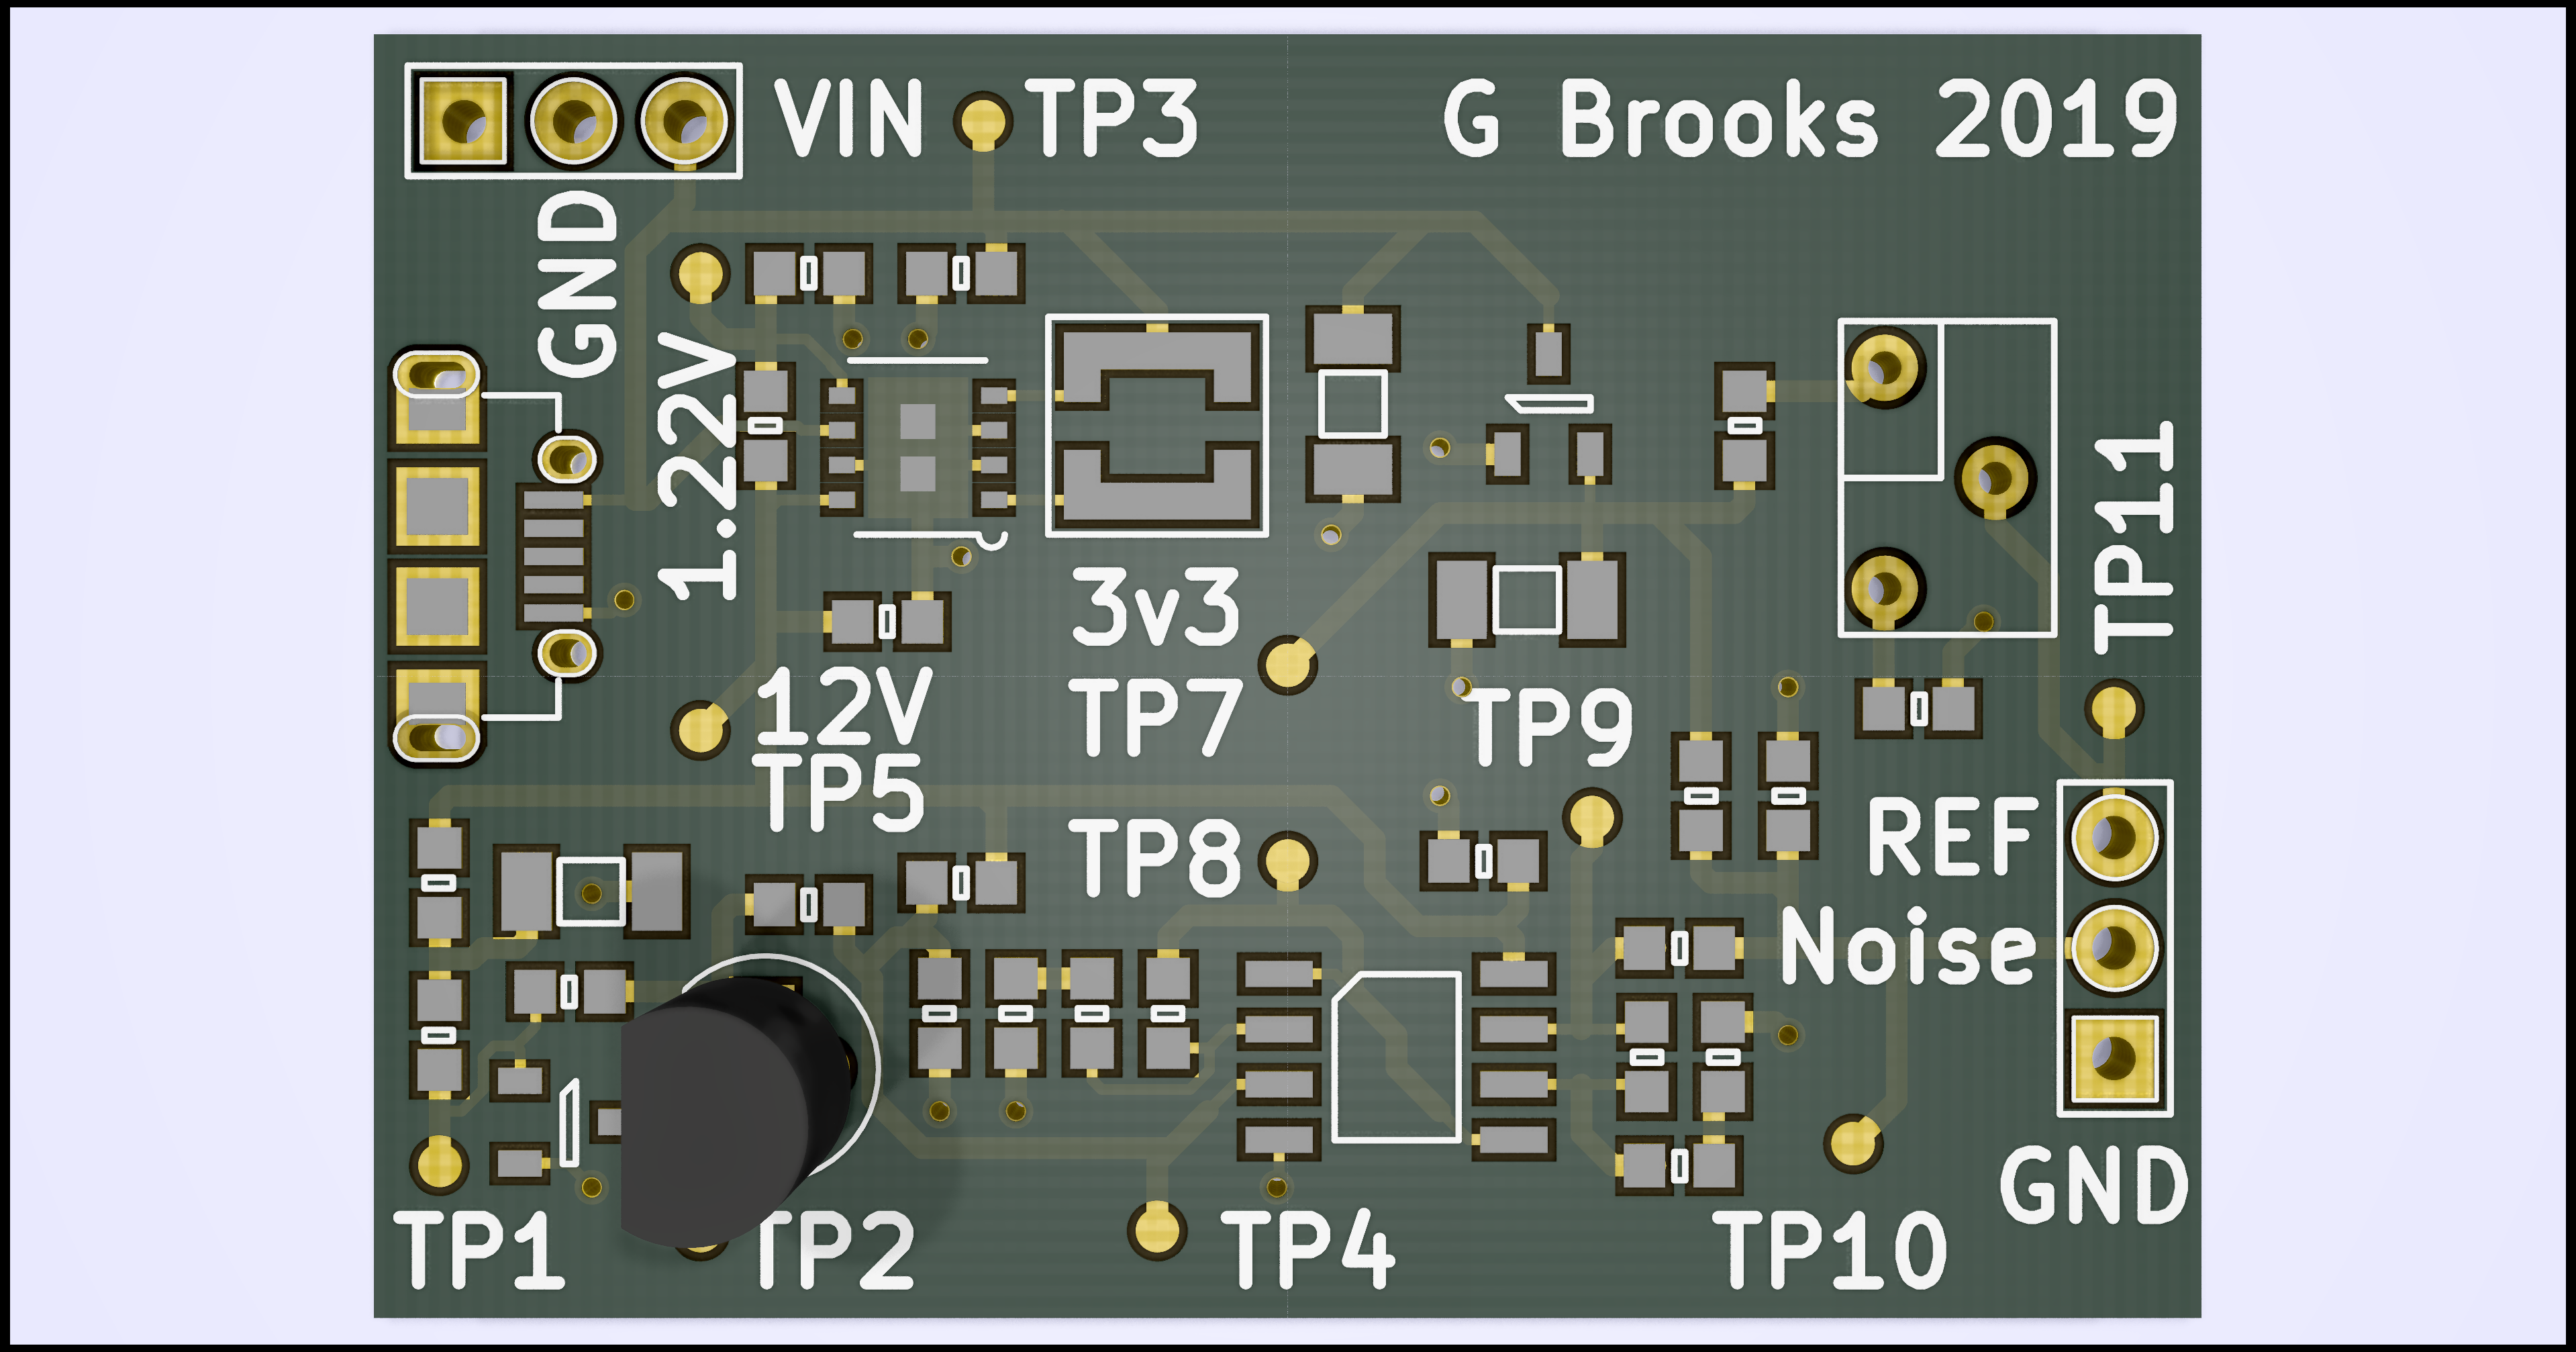
\includegraphics[width=0.4\textwidth]{fig/pcb_render_f.png}}
      \subfloat[Back]{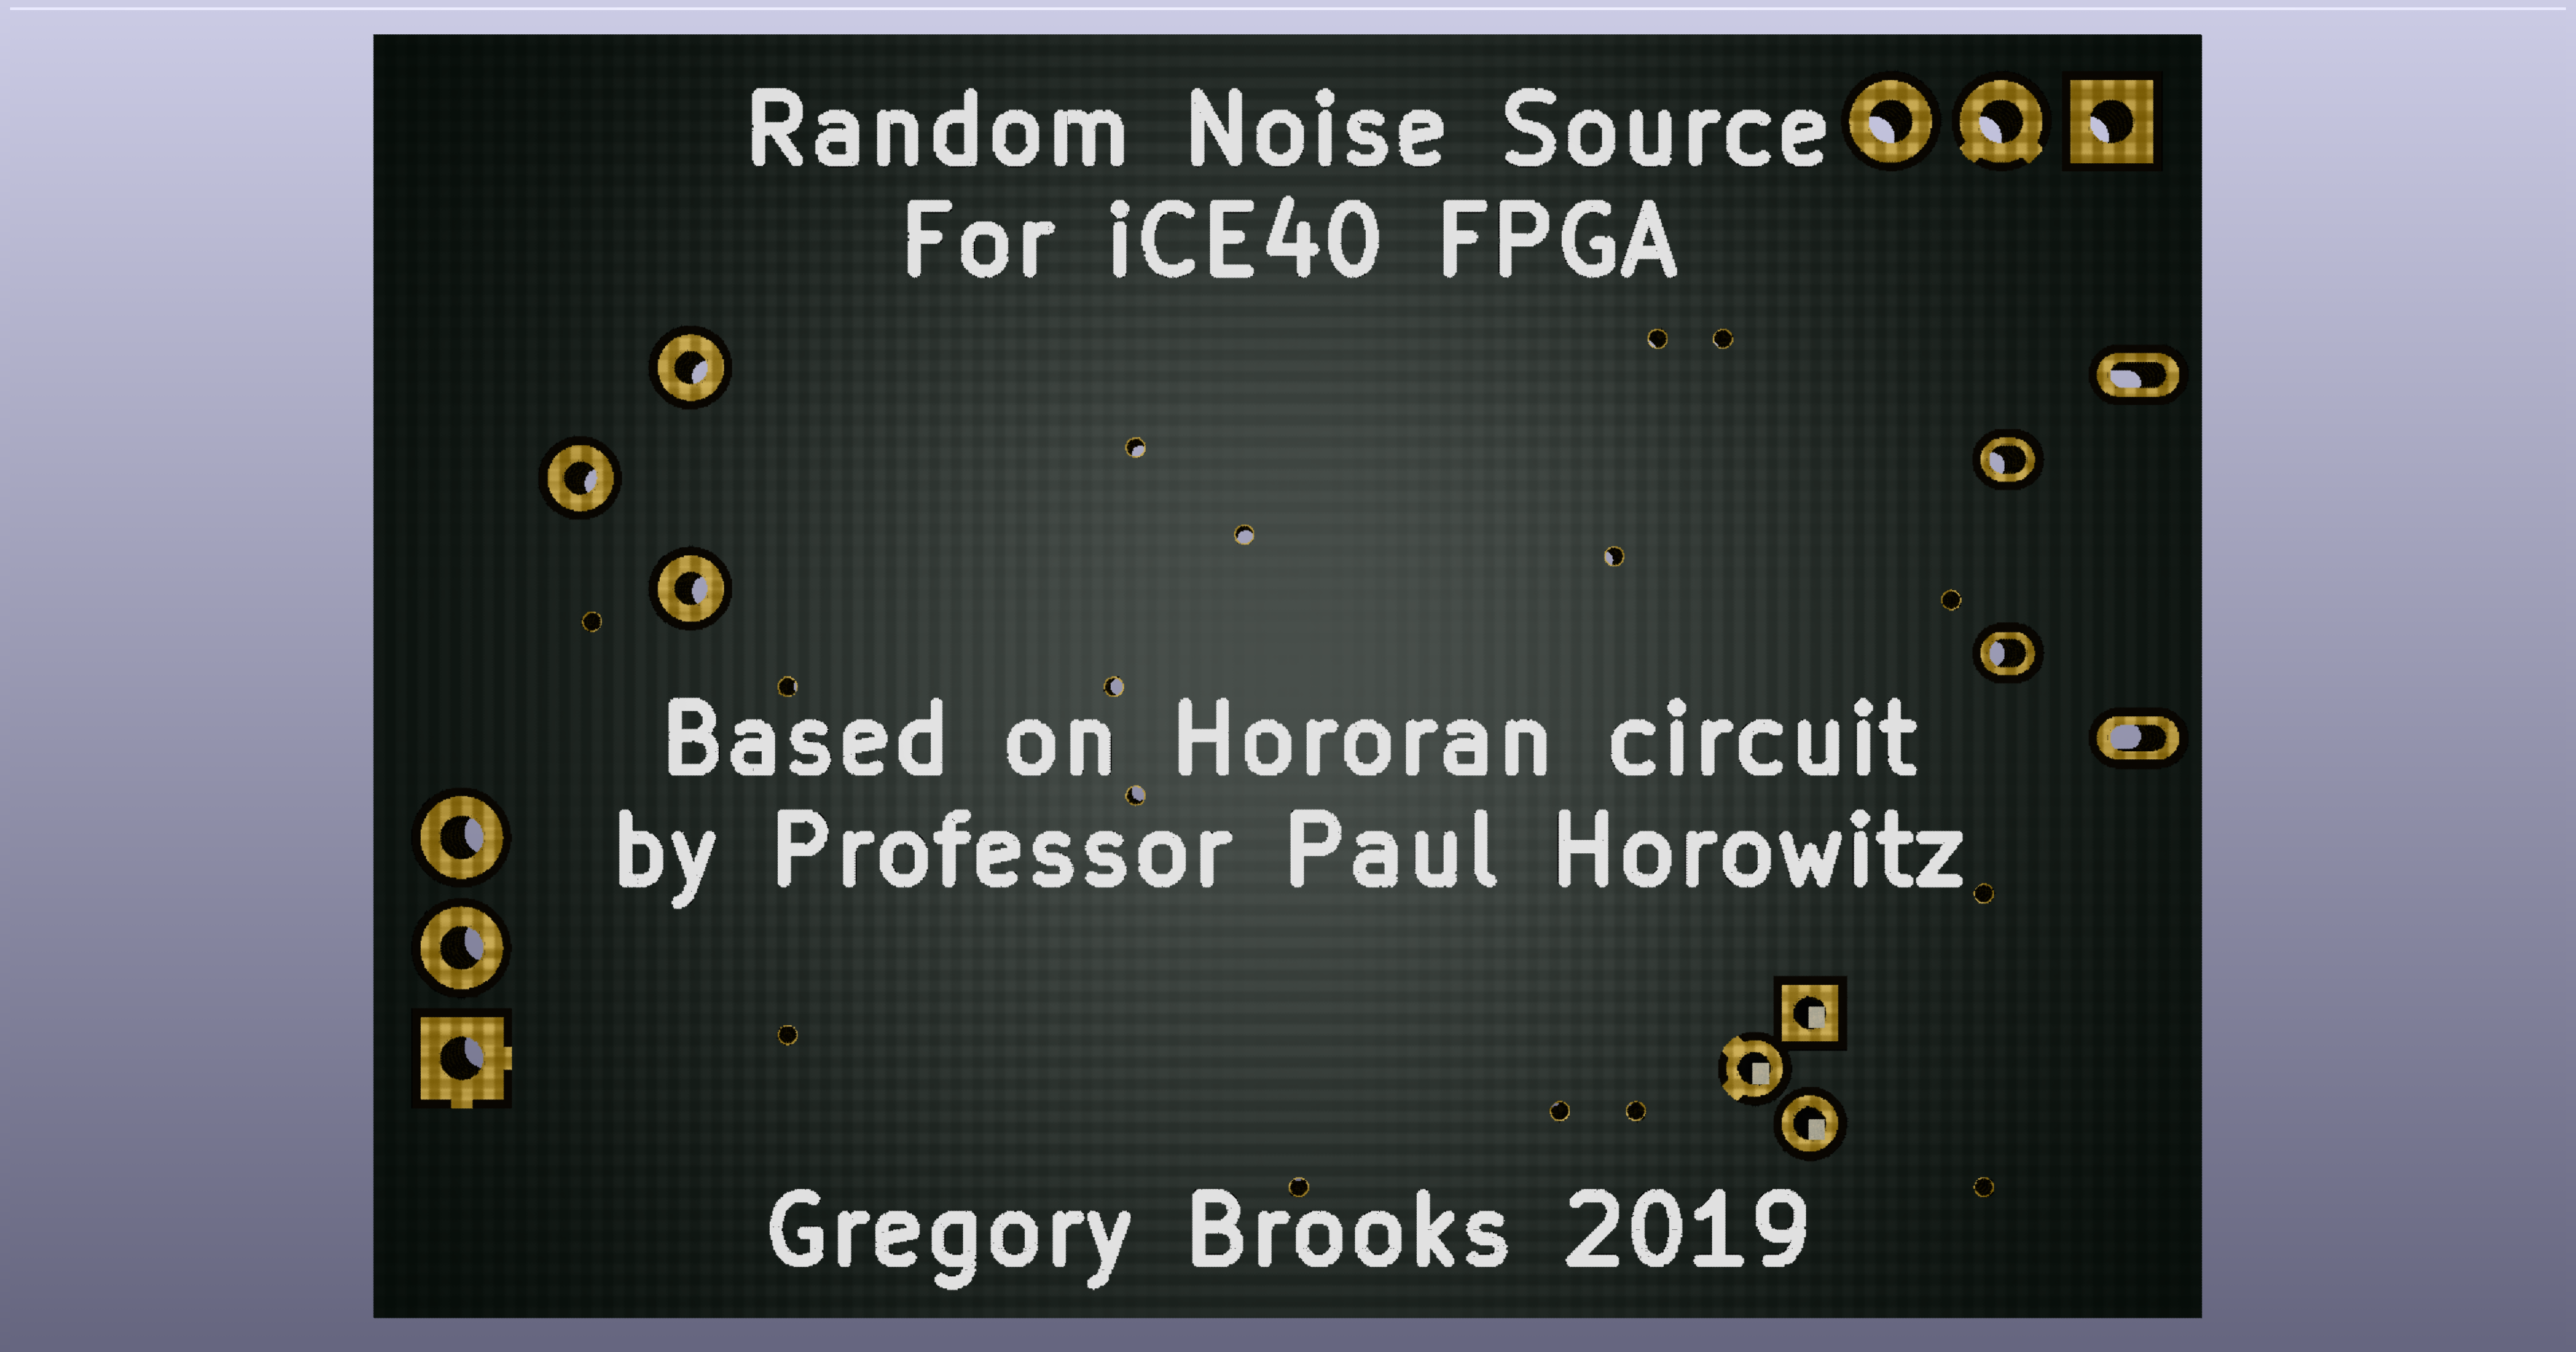
\includegraphics[width=0.4\textwidth]{fig/pcb_render_b.png}}
      \caption{3D renders of PCB (in KiCad).}
      \label{fig:pcb_render}
    \end{figure}

    \textit{$\langle$ TODO: finish$\rangle$}
    \\
    The full circuit schematic and PCB layout can be found in Appendix \ref{appendix:schematic}, as well as the GitHub repository listed in Section \ref{subsection:GitHub}.

      \subsubsection{Evaluation of Circuit Performance}

      \begin{figure}[H]
        \centering
        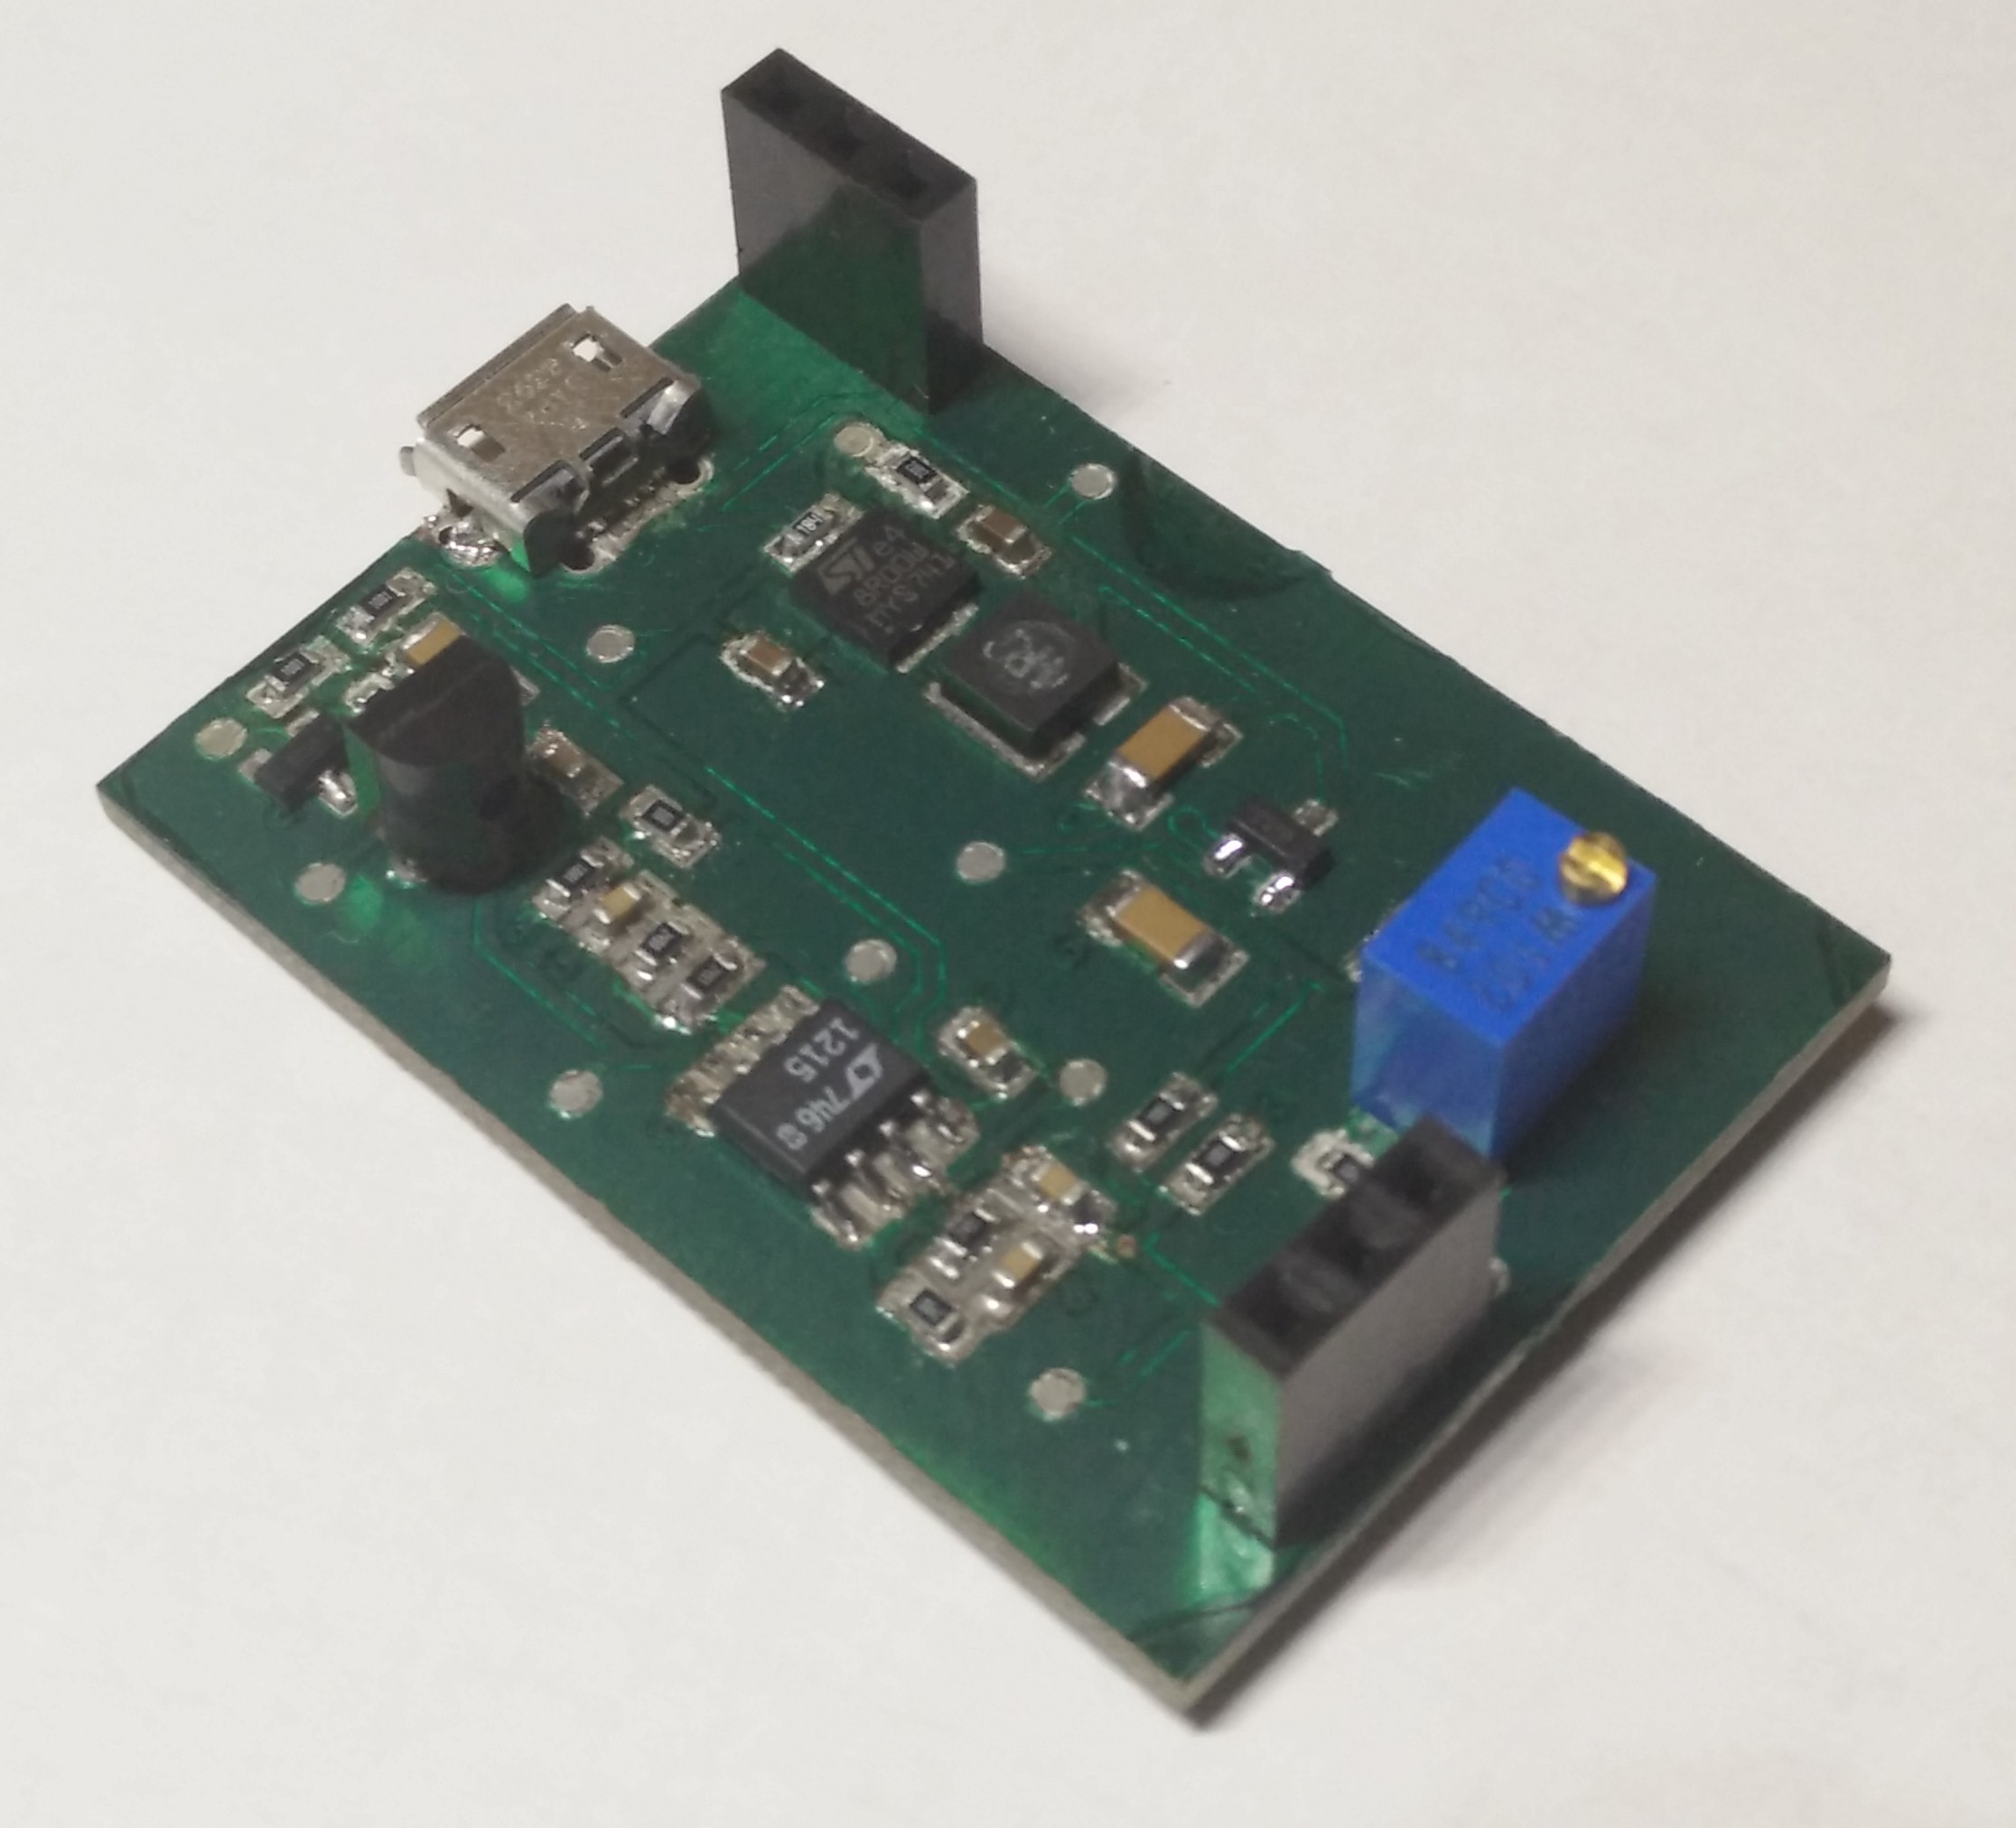
\includegraphics[width=0.5\textwidth]{fig/PCB_CROPPED.jpg}
        \caption{The physical PCB, assembled by the CUED Dyson Centre's Electronics Development Group.}
        \label{fig:pcb_cropped}
      \end{figure}

      \textit{$\langle$ TODO: finish e.g. talk about measured circuit specs (e.g. noise bandwidth)$\rangle$}\\
      \textit{$\langle$ TODO: include all measurements (put large figures in appendix)$\rangle$}

      One problem identified during testing was the tendency for the 12V boost regulator's inductor to get very hot during operation; whilst the circuit still functions in a room temperature environment, a further prototype iteration would use an inductor with a higher current rating to improve reliability. This might require a redesign of the PCB to accommodate a larger inductor package and footprint, although similarly sized alternatives are available\footnote{e.g. Coilcraft XAL4030-472MEC with a 5.1A RMS current rating, compared to the 1.2A for the Wurth Elektronik 744031004 currently being used. The datasheet for the ST8R00 step-up regulator states an absolute maximum inductor current of 3A~\cite{ST8R00}.}.

      \textit{$\langle$ TODO: calc theoretical inductor current (see graph in datasheet for example)$\rangle$}\\
      \textit{$\langle$ TODO: measure inductor voltage and hence inductor current - is it within spec?$\rangle$}


  \subsection{Uniform Random Number Generator}
  \textit{$\langle$ TODO: insert block diagram$\rangle$}

  \subsection{Inversion Method Random Number Generator}
    \textit{$\langle$ TODO: insert block diagram$\rangle$}



%
% RESULTS
%

\section{Results}

  \subsection{Scaling of Logic Implementations}
    \textit{$\langle$ TODO: investigate how URNG and RNG logic implementations scale with various parameters (and how this compares to a naive implementation)$\rangle$}

    \textit{$\langle$ TODO: investigate scaling of adder hardware (inferred from Verilog vs iCE40 hardware accumulators)$\rangle$}

  \subsection{Randomness of RNG Output}
    \textit{$\langle$ TODO: with and without zener diode$\rangle$}


\newpage



%
% CONCLUSIONS
%

\section{Conclusions}

\newpage



\noindent

% Hack to remove REFERENCES REFERENCES header
\markboth{}{}
\printbibliography
\markboth{}{}

\newpage

\begin{appendix}

  %
  % RISK ASSESSMENT RETROSPECTIVE
  %

  \section{Risk Assessment Retrospective}
    The risk assessment submitted at the start of the project does not mention any specific hazards besides office (computer) work, since the project is predominately software/firmware based (all project hardware operated at low voltages i.e. 12V or less). No other hazards were encountered during the course of the project, since the random noise generator PCBs were manufactured by the Dyson Centre's Electronics Development Group. In retrospect, although not part of the initial project specification, the risk assessment could have anticipated the possibility of manufacturing PCBs for the project. The hazards associated with this activity include high temperatures (from a soldering iron/oven/hot air gun) as well as chemical hazards associated with solder, fume extraction etc.



  %
  % UPPER BOUND ON DIFF PRIV
  %

  \section{Derivation of an Upper Bound on \textit{Indirect} Differential Privacy Loss} \label{appendix:diff_priv_loss}
    Let $\hat{X}$ be a random variable denoting a sensor measurement, including any measurement error.
    \\
    \\
    Let $N_{Laplace}^\lambda$ be a random variable following a Laplace distribution with parameter $\lambda$. This represents random noise added to sensor measurements.
    \\
    \\
    Let $X$ be a random variable representing a \textit{noised} sensor measurement i.e. the masked value that the differential privacy system provides to the outside world after applying Laplace distributed noise to a measurement:
    \begin{equation}
      X = \hat{X} + N_{Laplace}^\lambda
    \end{equation}
    A measurement event comprises the variable $\hat{X}$ taking on value $\hat{x}$. Similarly, a noising event can be defined by $X$ taking value $x = \hat{x} + n$. We define an embedded system as having $n$ sensors with measurements distributed as $\hat{X}_i$, $1 \leq i \leq n$.
    \\
    \\
    Let $Y$ denote a variable derived from one or more \textit{noised measurements}, $X$, such as measurements from different sensors in an embedded system:
    \begin{align*}
      Y & = f(X_1, X_2, ..., X_n) = f(\bf{X})\\
      y & = f(x_{1}, x_{2}, ..., x_{n}) = f(\bf{x})
    \end{align*}
    This same mapping function $f(\bf{x})$ can take unnoised measurements as arguments:
    \begin{align*}
      \hat{Y} & = f(\hat{X}_1, \hat{X}_2, ..., \hat{X}_n) = f(\bf{\hat{X}})\\
      \hat{y} & = f(\hat{x}_{1}, \hat{x}_{2}, ..., \hat{x}_{n}) = f(\bf{\hat{x}})
    \end{align*}
    Using this function, an untrusted party can compute an instance value $y$ by taking measurements $x_{1}$ to $x_{n}$ --- variable $\hat{Y}$ has experienced some privacy loss, $l_{\hat{Y}}$, since a noised instance value $y$ has effectively been released to the outside world (i.e. untrusted parties), revealing some information about the private noise-free value $\hat{y}$ taken by variable $\hat{Y}$. The privacy loss can be quantified using a log-likelihood ratio~\cite{Choi2018GuaranteeingLD} (Equation \ref{eqn:privacy_loss}). This privacy loss function requires two parameters,  $\hat{y}_a$ and $\hat{y}_b$, which are the possible \textit{true} i.e. noise-free values for $\hat{Y}$ that maximise the privacy loss (Equation \ref{eqn:argmax}).
    \begin{equation}
      y_{obs} = f(\bf{x}_{obs}) = \text{value for $y$ calculated from noised measurements $\bf{x}_i$} \nonumber\\
    \end{equation}
    \begin{align}
      % \bf{\hat{x}_a}, \bf{\hat{x}_b} & = \argmax_{\bf{\hat{x}_a}, \bf{\hat{x}_b}} l_{\hat{Y}}(\bf{\hat{x}_a}, \bf{\hat{x}_b}) \label{eqn:argmax}\\
      % l_{\hat{Y}}(\bf{\hat{x}_a}, \bf{\hat{x}_b}) & = log \left( \frac{Pr\{ Y = y_{obs} | \bf{\hat{X}} = \bf{\hat{x}_a} \}}{Pr\{ Y = y_{obs} | \bf{\hat{X}} = \bf{\hat{x}_b} \}} \right) \label{eqn:privacy_loss}
      \hat{y}_a, \hat{y}_b & = \argmax_{\hat{y}_a, \hat{y}_b} l_{\hat{Y}}(\hat{y}_a, \hat{y}_b) \label{eqn:argmax}\\
      l_{\hat{Y}}(\hat{y}_a, \hat{y}_b) & = log \left( \frac{Pr\{ Y = y_{obs} | \hat{Y} = \hat{y}_a \}}{Pr\{ Y = y_{obs} | \hat{Y} = \hat{y}_b \}} \right) \label{eqn:privacy_loss}
    \end{align}
    Equation \ref{eqn:privacy_loss} can be rewritten as follows, where $\bf{\hat{x}_a}$ and $\bf{\hat{x}_b}$ are chosen to maximise $l_{\hat{Y}}$ as before, but subject to constraints $\bf{\hat{x}_a}$ $ = f^{-1}(\hat{y}_a)$ and $\bf{\hat{x}_b}$ $ = f^{-1}(\hat{y}_b)$:
    \begin{align}
      l_{\hat{Y}}(\bf{\hat{x}_a}, \bf{\hat{x}_b}) & = log \left( \frac{Pr\{ \bf{X} = \bf{x}_{obs} | \bf{\hat{X}} = \bf{\hat{x}_a} \}}{Pr\{ \bf{X} = \bf{x}_{obs} | \bf{\hat{X}} = \bf{\hat{x}_b} \}} \right) \label{eqn:exact_indirect_priv_loss}
    \end{align}
    This constrained optimisation problem could be solved to calculate an exact value for privacy loss. Alternatively, an upper bound on privacy loss can be determined using a far simpler calculation (the sum of privacy losses for each individual sensor):
    \begin{align}
      l_{\hat{Y}}(\bf{\hat{x}_a}, \bf{\hat{x}_b}) & = log \left( \prod_{u=1}^n \frac{Pr\{ X_u = x_{u,obs} | \hat{X}_u = \hat{x}_{u,a} \}} {Pr\{ X_u = x_{u,obs} | \hat{X}_u = \hat{x}_{u,b} \}} \right) \nonumber \\
      & \leq log \left( \prod_{u=1}^n \frac{Pr\{ X_u = x_{u,obs} | \hat{X}_u = \hat{x}_{u,c} \}}{Pr\{ X_u = x_{u,obs} | \hat{X}_u = \hat{x}_{u,d} \}} \right) \label{eqn:upper_bound} \\
      \text{where:} & \nonumber \\
      & \hat{x}_{u,c} = \argmax_{\hat{x}_{u,c}}Pr\{ X_u = x_{u,obs} | \hat{X}_u = \hat{x}_{u,c} \} \nonumber \\
      & \hat{x}_{u,d} = \argmin_{\hat{x}_{u,d}}Pr\{ X_u = x_{u,obs} | \hat{X}_u = \hat{x}_{u,d} \} \nonumber
    \end{align}
    i.e. the constraint $f^{-1}(\hat{y})$ has been removed. Equation \ref{eqn:upper_bound} can be interpreted as the sum of the privacy losses incurred by the $X$ variables i.e. $\sum_{u=1}^n l_{X_u}$. $Pr\{ X_u = x_{u,obs} | \hat{X}_u = \hat{x}_u \}$ is simply the Laplace distribution of the noise applied to the measurement represented by $\hat{X}$, centred on value $\hat{x}$.\\

    Note that this privacy loss is incurred when all values $x_{1,obs}$ to $x_{n,obs}$ are provided to the outside world (i.e. the event where an attacker transitions from having no information to the system to being provided with $x_{1,obs}$ to $x_{n,obs}$); for each subsequent individual query response $x_{u,obs}$, the resulting privacy loss is only:
    \begin{align}
      l_{\hat{Y}}(\bf{\hat{x}_a}, \bf{\hat{x}_b}) & = log \left( \frac{Pr\{ X_u = x_{u,obs} | \hat{X}_u = \hat{x}_{u,a} \}} {Pr\{ X_u = x_{u,obs} | \hat{X}_u = \hat{x}_{u,b} \}} \right)
    \end{align}
     where values for $\bf{\hat{x}_a}$ and $\bf{\hat{x}_b}$ are the same as those used in Equation \ref{eqn:exact_indirect_priv_loss} (if calculating exact privacy loss) or Equation \ref{eqn:upper_bound} (if calculating an upper bound).\\

    Since the Newton language recently gained a mutual information operator, I attempted to factor mutual information into this calculation. Unfortunately, it appears that mutual information alone does not provide enough information to calculate indirect privacy loss --- the exact nature of the correlation between two (or more) random variables is required i.e. the conditional distribution for the unknown variable given known ones:
    \\
    \\
    Define $\hat{X}$ and $X$ as before and let $\hat{Y}$ be a random variable correlated with $\hat{X}$. Both $\hat{X}$ and $\hat{Y}$ can take values within some range (e.g. due to finite sensor precision):
    \begin{align*}
      \hat{X} \in R_{\hat{X}},\ \hat{Y} \in R_{\hat{Y}}
    \end{align*}
    The mutual information $I(\hat{X};\hat{Y})$ is defined as:
    \begin{align}
      I(\hat{X};\hat{Y}) = \int_{R_{\hat{Y}}} \int_{R_{\hat{X}}} p(\hat{X}, \hat{Y}) log \left( \frac{p(\hat{X}, \hat{Y})}{p(\hat{X})p(\hat{Y})} \right) d\hat{X} d\hat{Y}
    \end{align}
    where $p()$ denotes the probability density function for a random variable. I have been unable to insert this value into the privacy loss equation, however a value for privacy loss can be obtained if the conditional distribution of $\hat{X}$ given $\hat{Y}$ is known, as this allows the conditional distribution of $X$ given $\hat{Y}$ to be calculated:
    \begin{equation}
      Pr\{X = x | \hat{Y} = \hat{y}\} = \int_{R_{\hat{X}}}Pr\{X = x | \hat{X} = \hat{x}\} Pr\{\hat{X} = \hat{x} | \hat{Y} = \hat{y}\} d \hat{x} \label{eqn:p_x_given_y_hat}
    \end{equation}
    Equation \ref{eqn:p_x_given_y_hat} can be substituted into Equation \ref{eqn:priv_loss_y_hat_initial}, the formula for privacy loss incurred by $\hat{Y}$ as a result of observing a value $x_{obs}$ for $X$. This results in Equation \ref{eqn:priv_loss_y_hat_final}:

    \begin{align}
      l_{\hat{Y}}(\hat{y}_a, \hat{y}_b) & = log \left( \frac{Pr\{X = x_{obs} | \hat{Y} = \hat{y}_a\}}{Pr\{X = x_{obs} | \hat{Y} = \hat{y}_b\}} \right) \label{eqn:priv_loss_y_hat_initial} \\
      & = log \left( \frac{\int_{R_{\hat{X}}} Pr\{X = x_{obs}| \hat{X} = \hat{x}\} Pr\{\hat{X}=\hat{x}|\hat{Y} = \hat{y}_a\} d\hat{x} }{\int_{R_{\hat{X}}} Pr\{X = x_{obs}| \hat{X} = \hat{x}\} Pr\{\hat{X}=\hat{x}|\hat{Y} = \hat{y}_b\} d\hat{x} }\right) \label{eqn:priv_loss_y_hat_final}
    \end{align}
    for $\hat{y}_a, \hat{y}_b = \argmax_{\hat{y}_a, \hat{y}_b}(l_{\hat{Y}})$ as before.
  %
  % URNG BLOCK DIAGRAM
  %

  \section{Uniform Random Number Generator: Block Diagram}
    \textit{$\langle$ TODO: insert block diagram$\rangle$}


  %
  % INVERSION METHOD BLOCK DIAGRAM
  %

  \section{Inversion Method Random Number Generator: Block Diagram}
    \textit{$\langle$ TODO: insert block diagram$\rangle$}


  %
  % NOISE GENERATOR SCHEMATIC AND PCB LAYOUT
  %
  \newpage
  \section{Hardware Entropy Source Schematic and PCB} \label{appendix:schematic}
  \vspace{-1cm}
    \begin{figure}[H]
      \centering
      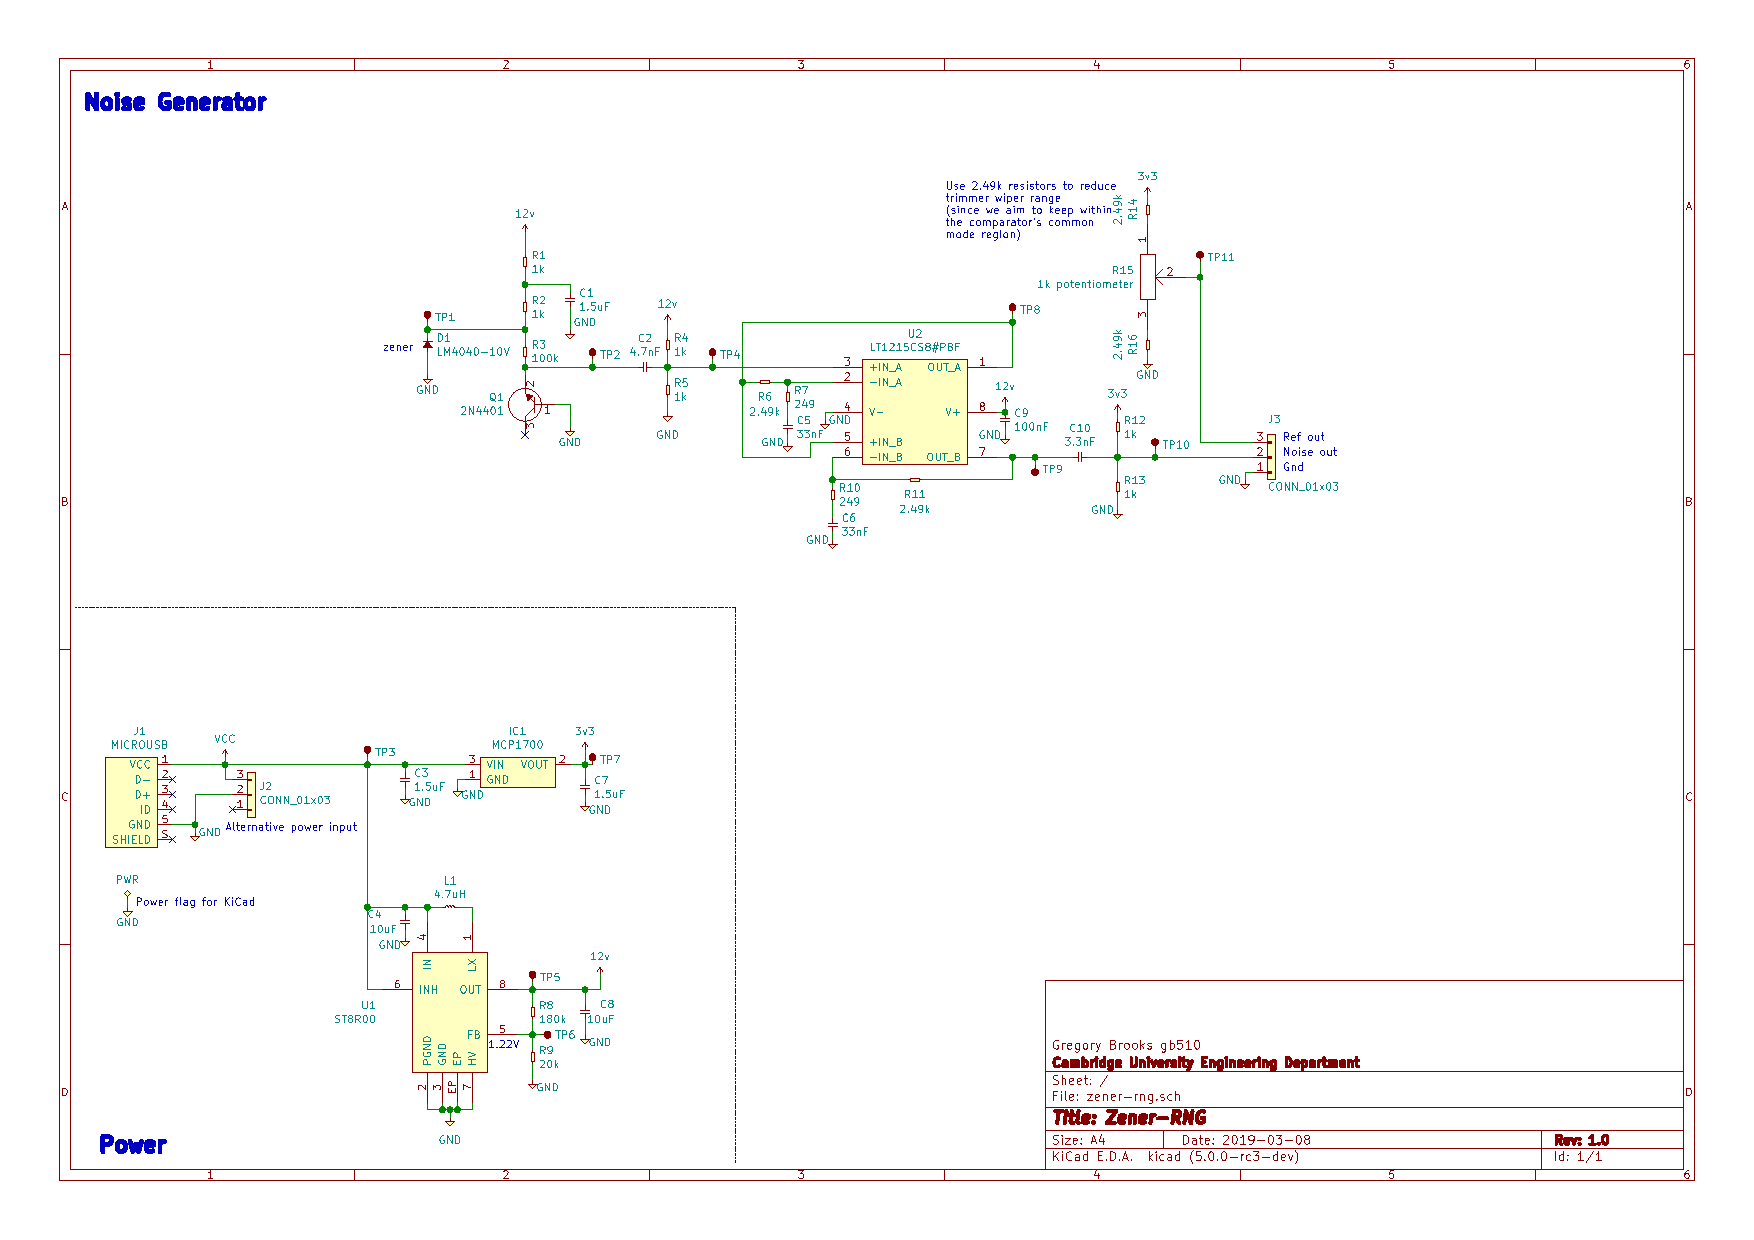
\includegraphics[angle=90,width=\textwidth]{fig/schematic.pdf}
      \label{fig:schematic}
    \end{figure}

    \newpage

    \vspace{-1.5cm}
    \begin{figure}[H]
      \centering
      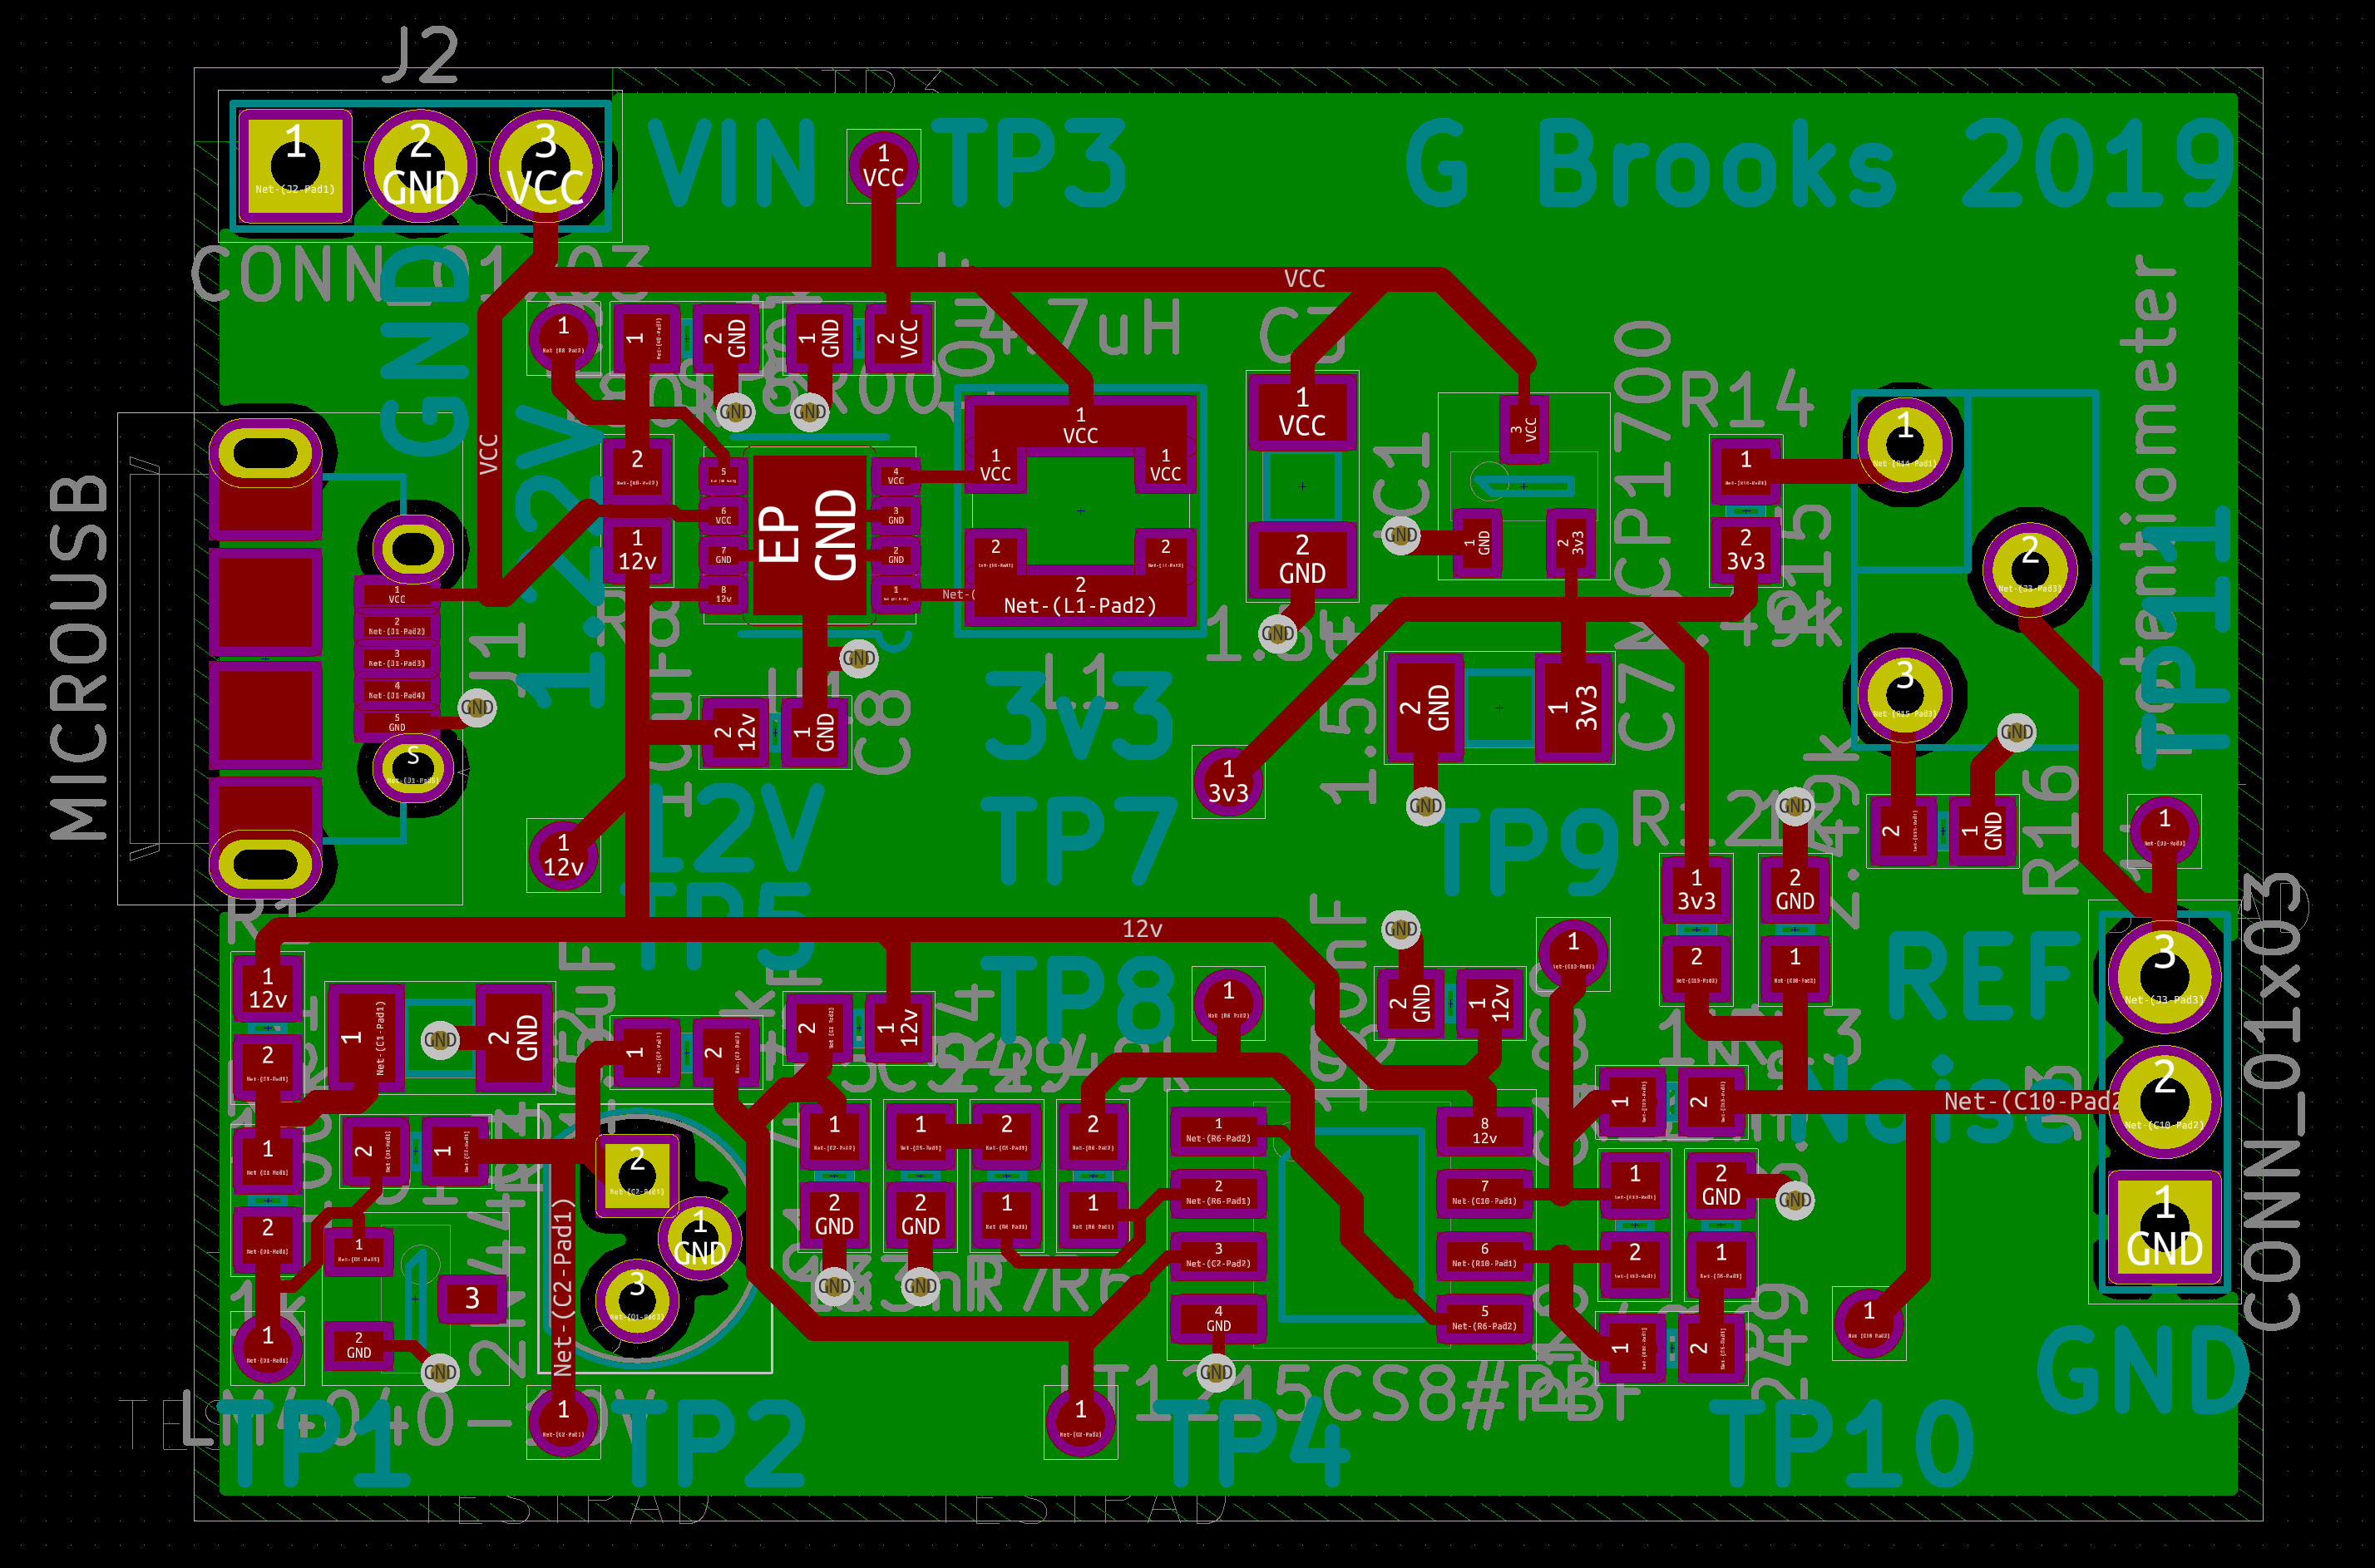
\includegraphics[angle=90, width=0.9\textwidth]{fig/pcb.PNG}
      \label{fig:pcb}
    \end{figure}

    \newpage

  %
  % EUROSYS POSTER
  %

  \section{EuroSys 2019 Poster: Safeguarding Sensor Device Drivers Using Physical Constraints}
    This poster~\cite{eurosys_poster} was submitted to EuroSys 2019, to communicate the idea of using information about a physical system to condition electronic sensor measurements. The example discussed in the poster is the detection and safeguarding against transduction attacks~\cite{Fu_2018}, where an attacker manipulates a sensor's output to gain control over a system. For example, research by Liu, Yan and Xu~\cite{autonomous_vehicles} has shown that the proximity sensors on a Tesla automobile can be fooled into providing erroneous (or even no) data using ultrasonic interference produced by a device built using off-the-shelf electronic components. An attacker is able to influence the system's behaviour without needing to directly manipulate the execution of the vehicle's firmware.\\

    The poster illustrates how the Newton language can be used to describe a physical system, in this case an accelerometer mounted to a PCB without vibration isolation. In this scenario, vibrations of the PCB (e.g. due to a nearby loudspeaker or even, in the case of a smartphone, due to loudspeakers mounted to the PCB) are measured by the accelerometer, obscuring a \textit{true} acceleration measurement i.e. acceleration of the entire system due to gravity. This effect is particularly pronounced if the board is driven at its resonant frequency, since the resulting oscillation will have a greater amplitude~\cite{adi}. This phenomenon could, in theory, be used as part of a transduction attack e.g. where a smartphone's loudspeaker is used to interfere with a software application's estimate of the device's physical orientation.\\

    To test whether this phenomenon can be distinguished from regular measurement noise, I performed an experiment~\cite{poster_experiment} using an MMA8451Q accelerometer mounted on an FRDM-KL03Z board. With the sensor resting stationary on a horizontal surface, five minutes worth of accelerometer samples were recorded at 10Hz in order to obtain a probability distribution for the accelerometer's measurement noise (along the z axis, aligned with the vertical); this data was empirically observed to fit a Laplace distribution. This measurement was then repeated with the board resting on top of a smartphone playing a 440Hz audio tone --- in theory, this data (random samples from a sinusoid) would fit a bimodal beta distribution (see section \ref{Poster_Derivation} for derivation) allowing a log likelihood ratio to be computed:

    \begin{equation}
      LLR = -2 \sum_{i = 1}^{N} \frac{\frac{1}{\pi}\left| \frac{1}{\sqrt{A^2\omega^4 - \ddot{x}_i^2}} \right|}{\frac{1}{2b} exp\left(-\frac{|\ddot{x}_i-\mu|}{b}\right)}
    \end{equation}

    The value of this log-likelihood ratio indicates whether the audio tone based transduction attack described here is likely to be occuring. For the data collected in the experiment, the log-likelihood ratio was found to be around -24600.08 whilst the tone was playing, and +3731 when it was not; the negative value indicates that the measurements taken whilst the tone was playing were indeed more accurately described by the bimodal beta distribution, compared to the Laplace distribution of sensor noise, and vice versa for the positive value.

    \subsection{Derivation of Bimodal Beta Distribution} \label{Poster_Derivation}
    Let T be a uniformly distributed random variable representing the time at which acceleration is sampled:
    \begin{align}
      T & \sim U\left(-\frac{\pi}{\omega}, \frac{\pi}{\omega}\right) \nonumber \\
      f_T(t) & =
        \begin{cases}
          \frac{\omega}{2\pi} & -\frac{\pi}{\omega} \leq t \leq \frac{\pi}{\omega}\\
          0 & \text{otherwise}
        \end{cases}\\
      F_T(t) & =
        \begin{cases}
          0 & t < -\frac{\pi}{\omega}\\
          \frac{\omega (t + \pi / \omega)}{2\pi} & -\frac{\pi}{\omega} \leq t \leq \frac{\pi}{\omega}\\
          1 & t > \frac{\pi}{\omega}
        \end{cases}
    \end{align}
    Then let X = g(T) represent the acceleration value at time T. By considering the dynamics of the system, we know that:

    \begin{equation}
      g(t) = A \omega^2 sin(\omega t)
    \end{equation}
    where A is a frequency-dependent constant equal to the product of quality factor and board displacement at resonance. We can also define a monotonically increasing function $h(x)$ as the inverse of $g(t)$:

    \begin{equation}
      h(x) = g^{-1}(x) = \frac{1}{\omega} arcsin \left(\frac{x}{A\omega^2}\right)
    \end{equation}
    \\
    The cumulative distribution function for X can therefore be written in terms of the cumulative distribution function for T, accounting for the fact that g(t) is not monotonic:
    \begin{equation}
      F_X(x) = F_T(h(x)) + \Big(1 - F_T(\pi/\omega - h(x))\Big)
    \end{equation}
    \\
    Taking the derivative results in the probability density function for X:
    \begin{align}
      f_X(x) & = \Big(f_T(h(x) - f_T(-h(x)))\Big) \frac{d(h(x))}{dx}\\
      & =
      \begin{cases}
        \frac{1}{\pi \sqrt{A^2 \omega^4 - x^2}} & |x| \leq A \omega^2\\
        0 & \text{otherwise}
      \end{cases}
    \end{align}

\end{appendix}

\end{document}
